\documentclass[a4paper,12pt]{article}
\usepackage[T1]{fontenc}
\usepackage[utf8]{inputenc}
\usepackage{graphicx}
\usepackage{lmodern}
\usepackage[czech]{babel}
\usepackage[T1]{fontenc}
\usepackage[utf8]{inputenc}
\title{UIR Seminární práce}
\usepackage{listings}
\usepackage{color}
\usepackage{hyperref}
\author{Jan František Sedláček}

\iffalse
#popis (zadání) problému
analýza problému
návrh řešení
popis řešení
uživatelská dokumentace
závěr
\fi


\definecolor{dkgreen}{rgb}{0,0.6,0}
\definecolor{gray}{rgb}{0.5,0.5,0.5}
\definecolor{mauve}{rgb}{0.58,0,0.82}

\lstset{frame=tb,
  language=Java,
  aboveskip=3mm,
  belowskip=3mm,
  showstringspaces=false,
  columns=flexible,
  basicstyle={\small\ttfamily},
  numbers=none,
  numberstyle=\tiny\color{gray},
  keywordstyle=\color{blue},
  commentstyle=\color{dkgreen},
  stringstyle=\color{mauve},
  breaklines=true,
  breakatwhitespace=true,
  tabsize=3
}

\begin{document}

\clearpage\maketitle
\thispagestyle{empty}

\begin{center}
  
\includegraphics[width=150px]{logo1.jpeg}
\end{center}

\pagebreak

\tableofcontents
\pagebreak

\section{Problematika}
\subsection{Zadání}
\paragraph{}
Ve zvoleném programovacím jazyce navrhněte a implementujte program, který umožní
klasifikovat textové dokumenty do tříd podle jejich obsahu, např. počasí, sport, politika,
apod.
\subsection{Analýza}
\paragraph{}
Řešení komplexní úlohy jako je strojové učení pro klasifikaci lze rozdělit na dílčí kroky 

\begin{itemize}
  \item Výběr programovacího jazyka
  \item Výběr vhodných algorithmů
  \item Samotná implementace řešení
  \item Testovaní a cross-validace výsledků
\end{itemize}

\subsubsection{Zvolený programovací jazyk}
\paragraph{}
Jako zvolený jazyk pro implementaci programu byla vybrána \textsf{java} ve verzi \textsf{11},
o proti jiným jazykům například \textsf{C} nebo \textsf{C++}, sice výkonostně zaostává ale rychlé 
čtění a zpracování textových souborů jsou při úloze ve které je očekávána práce s velkým množstvím
těchto dat velkou výhodou.
\paragraph{}
Úloha nevyžaduje složitejší UI proto bylo zvoleno \textsf{swing}, jedná se grafickou nadstavbu \textsf{javy}
a hlavní výhodou je urychlení rychlosti práce.
\paragraph{}
Nebyly použity žádné jiné externí nebo nestandartní knihovny 
\pagebreak
\subsubsection{Algoritmy}
Popis jednotlivých vybraných algoritmů
\paragraph{Najivní Bayes}
\subparagraph*{}
Naivní bayesovská klasifikace je druh jednoduchého pravděpodobnosti bayesovské klasifikace vychází z Bayesova teorému se silnou (tzv naivní) nezávislost hypotéz. Naivní Bayesův klasifikátor nebo Bayesův naivní klasifikátor, patří do rodiny lineárních klasifikátorů.
\subparagraph*{}
Vhodnějším termínem pro základní pravděpodobnostní model by mohl být „model se statisticky nezávislými charakteristikami“.
\subparagraph*{}
Jednoduše řečeno, naivní Bayesovský klasifikátor předpokládá, že existence charakteristiky třídy je nezávislá na existenci dalších charakteristik.
Například: 
Ovoce lze považovat za jablko, je-li červené, zaoblené a asi deset centimetrů veliké. I když jsou tyto vlastnosti ve skutečnosti spojeny, naivní Bayesovský klasifikátor určí, že ovoce je jablko, a to nezávisle na těchto vlastnostech barvy, tvaru a velikosti.
\paragraph{K-NN}
\subparagraph*{}
k-NN je neparametrickou metodou používanou pro klasifikaci a regresi. V obou případech jde o klasifikaci záznamu do kategorie, do které patří nejbližší sousedé k, do prostoru charakteristik identifikovaných učením. Výsledek závisí na tom, zda se algoritmus používá pro účely klasifikace nebo regrese:
\subparagraph*{}
Ve třídě k-NN je výsledkem třída členství. Vstupní objekt je klasifikován podle většinového výsledku statistiky třídy členství svých nejbližších sousedů ( k je obecně malé kladné celé číslo). Pokud k = 1, pak je objekt přiřazen ke třídě členství svého blízkého souseda.
v regresi k-NN je výsledkem hodnota tohoto objektu. Tato hodnota je průměrem hodnot k nejbližších sousedů.
Metoda k-NN je založena na předchozím učení nebo slabém učení, kde je funkce hodnocena lokálně, přičemž konečný výpočet se provádí na konci klasifikace. Algoritmus k -NN patří mezi nejjednodušší z algoritmů strojového učení.

\pagebreak
\subsubsection{Implementace}
\paragraph*{Datová reprezentace}
\subparagraph*{Bag of words}
Zjednodušená reprezentace používaná při zpracování přirozeného jazyka a při získávání informací . V tomto modelu je text (fráze nebo dokument) reprezentován jako množina jeho slov („bag“), bez ohledu na gramatickou strukturu a dokonce i na jejich seřazení, při zachování jejich multiplicity.
\begin{lstlisting}
// bag of words Naive bayes vyhodnoceni
 for(HashMap.Entry<String, Integer> entry : bag.getBagHashMap().entrySet())
        {
            String key = entry.getKey();

            for (BagOfWords bag1: trainedClasses)
            {
                if (bag1.countOccurrences(key)>0)
                {
                    double pX=bag.countOccurrences(key);

                    double pY=(bag.getBagHashMap().size());

                    double z=(pX/pY);

                    double pX2=bag1.countOccurrences(key);

                    double pY2=(bag1.getBagHashMap().size());

                    double z2=(pX2/pY2);

                    double c=z*z2;

                    bag1.setWeight( bag1.getWeight() + c);

                }

            }

        }

\end{lstlisting}
\pagebreak
\subparagraph*{IDF}
Nezpracovaná“ frekvence termínu je jednoduše počet výskytů tohoto termínu v uvažovaném dokumentu (mluvíme o „frekvenci“ jazyka).
\begin{lstlisting}
// Naive Bayes IDF vyhodnoceni
    for(HashMap.Entry<String, Integer> entry : bag.getBagHashMap().entrySet())
        {
            String key = entry.getKey();

            for (IDF bag1: trainedClasses)
            {
                for (Word w:bag1.getWordsSets().getWordList())
                {
                    if (w.getValue().equals(key))
                    {
                        bag1.setWeight(bag1.getWeight()+w.getFreq());
                        bag1.setFileCount(bag1.getFileCount()+1);
                    }
                }

            }

        }
\end{lstlisting}
\pagebreak
\subparagraph*{TFIDF}
Numerická míra, která vyjadřuje relevanci slova pro dokument ve sbírce. Tato reprezentace se často používá jako váhový faktor při získávání informací a těžbě textu. Hodnota tf-idf se úměrně zvyšuje, kolikrát se slovo v dokumentu objeví, ale zárověň je kompenzováno frekvencí slova ve sbírce dokumentů.
\begin{lstlisting}
//Naive Bayes TFIDF vyhodnoceni
   for(HashMap.Entry<String, Integer> entry : bag.getBagHashMap().entrySet())
        {
            String key = entry.getKey();

            for (TFIDF bag1: trainedClasses)
            {
                for (Word w:bag1.getWordsSets().getWordList())
                {
                    if (w.getValue().equals(key))
                    {
                        bag1.setWeight(bag1.getWeight()+w.getFreq());
                        bag1.setFileCount(bag1.getFileCount()+1);
                    }
                }

            }

        }
\end{lstlisting}

\pagebreak
\section{Testování}
\subsection{Testovací data}
Program byl testován na několika korpuses s několika různých oborů
\begin{itemize}
  \item Základní zadaný korpus (historické noviny) dále je korpus
   \begin{itemize}
  \item Zadaný předanatovaný soubor starých novinových článků
  \begin{itemize}
    \item pol
    \item kul
    \item err
    \item ...
  \end{itemize}
    \end{itemize}
  \item Jazykové rozpoznání (články z \url{wikipedia.org} v různých jazycích)
  \begin{itemize}
  \item několik odborných článků z různých oborů v různých jazycích sloužící k rozpoznání jazyků
  \begin{itemize}
    \item cs (Čeština)
    \item en (Angličtina)
    \item ge (Němčina)
  \end{itemize}
  \end{itemize}
  \item Reuters korpus (články z portálu reuters rok 1987)
   \begin{itemize}
  \item Staré reuters články ve formátu sgm s několika možnostmi klasifikace (topics, places, writers)
   \begin{itemize}
    \item earn
    \item oil
    \item oil-palm
    \item ...
  \end{itemize}
  \end{itemize}
  \item Rozpoznání moderních novin (Články z portálu \url{novinky.cz})
  \begin{itemize}
  \item novodobé novinové články ze tří katogorií 
   \begin{itemize}
    \item krimi
    \item sport
    \item pol (politika)
  \end{itemize}
    \end{itemize}
\end{itemize}
\subsection{Postup}
\begin{enumerate}
  \item Data pro testování jsou nahrána do vyrovnávací paměti pro testovací data
  \item Program je naučen jednotlivě 6 algoritmů
  \item Ručně je testováno několik souborů pro kontrolu nahrání dat
  \item Automaticky je vyhodnocený zbytek dat, výsledkem je přesnost  
\end{enumerate}
\subsubsection{Přesnost}
\texttt{Cn = celkový počet tříd}
\linebreak
\texttt{Ci = na jaké pozici byla určena první správná třída}
\linebreak
\linebreak
$ACC=\frac{\sum(100/Ci^{2})}{Cn}$
\subsection{Výsledky}
\subsubsection{Korpus}
\begin{itemize}
    \item Bag of world 
\begin{itemize}
    \item Naive Bayes = 66[\%]
    \item IDF = 13[\%]
    \item TF-IDF = 14[\%]
\end{itemize}
    \item K-NN 
\begin{itemize}
    \item Naive Bayes = 66[\%]
    \item IDF = 15[\%]
    \item TF-IDF = 14[\%]
\end{itemize}
\end{itemize}
Trace
\begin{lstlisting}[language=bash]
Classes File loaded: 21
Train File loaded: 412
Bag of Word Created
IDF Created
TF-IDF Created
Test File loaded: 99
Test File loaded: 99
\end{lstlisting}
\subsubsection{Wiki jazyky}
\begin{itemize}
    \item Bag of world 
\begin{itemize}
    \item Naive Bayes = 100[\%]
    \item IDF = 66[\%]
    \item TF-IDF = 54[\%]
\end{itemize}
    \item K-NN 
\begin{itemize}
    \item Naive Bayes = 100[\%]
    \item IDF = 66[\%]
    \item TF-IDF = 54[\%]
\end{itemize}
\end{itemize}
Trace
\begin{lstlisting}[language=bash]
Classes File loaded: 3
Train File loaded: 19
Bag of Word Created
IDF Created
TF-IDF Created
Test File loaded: 19
\end{lstlisting}
\subsubsection{NovinkyCZ}
Testováno ručně. Články brány z portálu \url{ct24.cz}. Převážně lépe vyhodnocovali IDF a TFIDF.
\subsubsection{Reuters}
Kvůli velkému množstí dat a podobě souborů je učení a testování extrémně zdlouhavý proces
\section{Uživatelská příručka}
  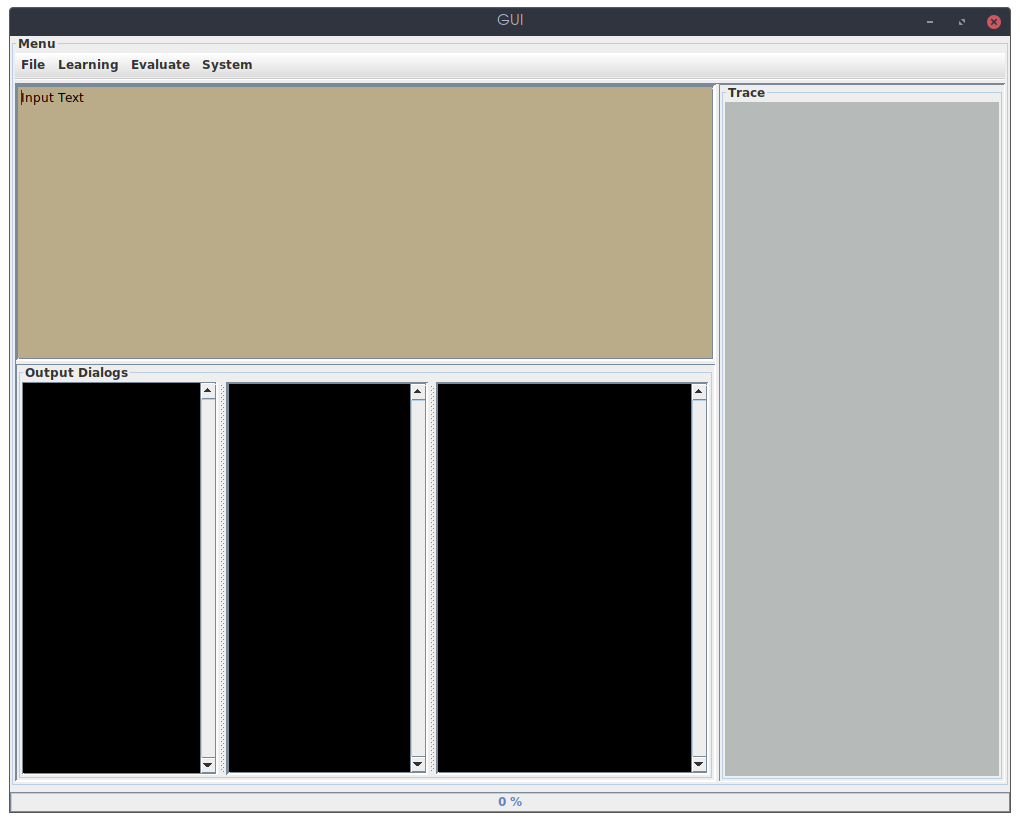
\includegraphics[width=400px]{main.png}
  Položky menu
  \begin{itemize} 
    \item File
    \begin{itemize}
      \item Save ... (uložení modulů) 
      \item Read ... (načtení modulů)
    \end{itemize}
    \item Learning
    \begin{itemize}
      \item Learn ... (učení podle načtených dat !!nejdříve je třeba načíst data!!)
      \item Read Train Data (spustí dialog pro načtení dat pro učení)
    \end{itemize}
    \item Evaluate
    \begin{itemize}
      \item ... [Textbox input] (vyhodnotí ručně zadaný text)
      \item ... [Accuracy Test] (spustí dialog pro automatické testovaní)
    \end{itemize}
    \item System
    \begin{itemize}
      \item Clear Trace (vymaže logy)
      \item Realtime testing "..." (spustí nebo ukončí automatické vyhodnocování ručně zadaného textu)
      \item Exit (ukončí program)
    \end{itemize}
  \end{itemize}
  Output Dialogs
  \begin{itemize}
    \item dialogová okna zobrazující výsledky
  \end{itemize}
  Trace
  \begin{itemize}
    \item logovací okno
  \end{itemize}
  \pagebreak
\section{Závěr}

Výsledné procenta nebyla scela podle očekávání především u IDF a TFIDF. Při změně testovacích dat se ukázalo že IDF a TFIDF jsou více závislé na velikosti trénovací množiny a u TFIDF také počtů jednotlivých dokumenků. Naivní Bayes se ukázal jako o něco méně přesnější než K-NN ale minimálně v jazyce Java byl výkonostně lepší ovšem nedá se z toho vyvodit v tomto ohledu žádný závěr, protože by muselo dojít k testům na více jazycích a to není účelem této práce. Program nicméně splnuje základní požadavky. Vylepšení by mohlo přijít v podobě přesnějších algoritmů, vylepšení UI nebo přidání české lokalizace.

\end{document}
